\chapter{Specifikacija programske potpore}
		
	\section{Funkcionalni zahtjevi}
			
			\textbf{\textit{dio 1. revizije}}\\
			
			\textit{Navesti \textbf{dionike} koji imaju \textbf{interes u ovom sustavu} ili  \textbf{su nositelji odgovornosti}. To su prije svega korisnici, ali i administratori sustava, naručitelji, razvojni tim.}\\
				
			\textit{Navesti \textbf{aktore} koji izravno \textbf{koriste} ili \textbf{komuniciraju sa sustavom}. Oni mogu imati inicijatorsku ulogu, tj. započinju određene procese u sustavu ili samo sudioničku ulogu, tj. obavljaju određeni posao. Za svakog aktora navesti funkcionalne zahtjeve koji se na njega odnose.}\\
			
			
			\noindent \textbf{Dionici:}
			
			\begin{packed_enum}
				
				\item Dionik 1
				\item Dionik 2				
				\item ...
				
			\end{packed_enum}
			
			\noindent \textbf{Aktori i njihovi funkcionalni zahtjevi:}
			
			
			\begin{packed_enum}
				\item  \underbar{Aktor 1 (inicijator) može:}
				
				\begin{packed_enum}
					
					\item funkcionalnost 1
					\item funkcionalnost 2
					\begin{packed_enum}
						
						\item  podfunkcionalnost 1 
						\item  podfunkcionalnost 2
				
					\end{packed_enum}
					\item  funkcionalnost 3
					
				\end{packed_enum}
			
				\item  \underbar{Aktor 2 (sudionik) može:}
				
				\begin{packed_enum}
					
					\item funkcionalnost 1
					\item funkcionalnost 2
					
				\end{packed_enum}
			\end{packed_enum}
			
			\eject 
			
			
				
			\subsection{Obrasci uporabe}
				
				\textbf{\textit{dio 1. revizije}}
				
				\subsubsection{Opis obrazaca uporabe}
					\textit{Funkcionalne zahtjeve razraditi u obliku obrazaca uporabe. Svaki obrazac je potrebno razraditi prema donjem predlošku. Ukoliko u nekom koraku može doći do odstupanja, potrebno je to odstupanje opisati i po mogućnosti ponuditi rješenje kojim bi se tijek obrasca vratio na osnovni tijek.}\\
					

					\noindent \underbar{\textbf{UC$<$broj obrasca$>$ -$<$ime obrasca$>$}}
					\begin{packed_item}
	
						\item \textbf{Glavni sudionik: }$<$sudionik$>$
						\item  \textbf{Cilj:} $<$cilj$>$
						\item  \textbf{Sudionici:} $<$sudionici$>$
						\item  \textbf{Preduvjet:} $<$preduvjet$>$
						\item  \textbf{Opis osnovnog tijeka:}
						
						\item[] \begin{packed_enum}
	
							\item $<$opis korak jedan$>$
							\item $<$opis korak dva$>$
							\item $<$opis korak tri$>$
							\item $<$opis korak četiri$>$
							\item $<$opis korak pet$>$
						\end{packed_enum}
						
						\item  \textbf{Opis mogućih odstupanja:}
						
						\item[] \begin{packed_item}
	
							\item[2.a] $<$opis mogućeg scenarija odstupanja u koraku 2$>$
							\item[] \begin{packed_enum}
								
								\item $<$opis rješenja mogućeg scenarija korak 1$>$
								\item $<$opis rješenja mogućeg scenarija korak 2$>$
								
							\end{packed_enum}
							\item[2.b] $<$opis mogućeg scenarija odstupanja u koraku 2$>$
							\item[3.a] $<$opis mogućeg scenarija odstupanja  u koraku 3$>$
							
						\end{packed_item}
					\end{packed_item}
				
					
				\subsubsection{Dijagrami obrazaca uporabe}
					
					\textit{Prikazati odnos aktora i obrazaca uporabe odgovarajućim UML dijagramom. Nije nužno nacrtati sve na jednom dijagramu. Modelirati po razinama apstrakcije i skupovima srodnih funkcionalnosti.}
				\eject		
				
				\subsection{Sekvencijski dijagrami}
				
				\textbf{Obrazac uporabe UC4 - Prijava nestale osobe}
    
                Klijent šalje zahtjev za prijavu nestale osobe. Poslužitelj prikazuje obrazac za prijavu. Klijent ispunjava obrazac (ime, prezime, fotografija i opis) za prijavu nestale osobe. Poslužitelj dohvaća podatke iz baze te provjerava je li nova prijavljena osoba u bazi. Ako osoba dosad nije prijavljena, zapisuje se u bazu nestalih te sustav šalje potvrdu i prikaz prijave. Ukoliko je osoba već prijavljena, poslužitelj obavještava klijenta uz poruku.

                \begin{figure}[H] 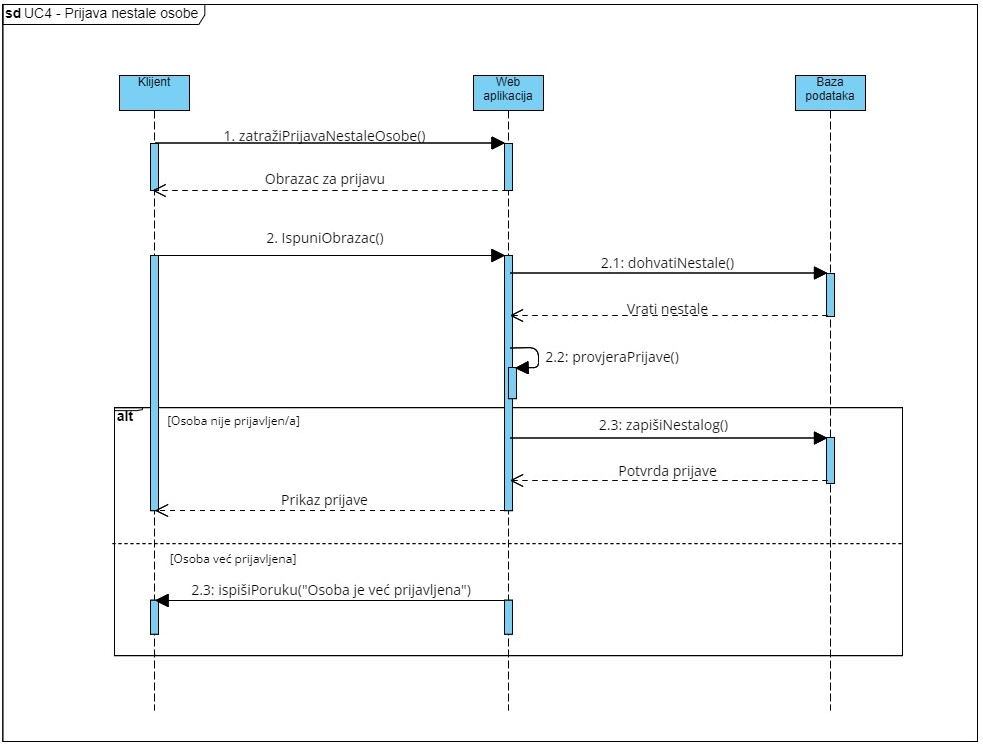
\includegraphics[width=\linewidth]{./dijagrami/PrijavaNestalog.jpg}
				    \caption{Sekvencijski dijagram za UC4 - Prijava nestale osobe}
				    \end{figure}

                \eject

                \textbf{Obrazac uporabe UC10 - Stvaranje operacije}

                Klijent šalje zahtjev za stvaranje operacije. Sustav provjerava je li korisnik voditelj. Ako korisnik nije voditelj, poslužitelj će ispisati poruku da nema ovlaštenje za stvaranje nove operacije, a ukoliko je, poslat će obrazac za stvaranje nove operacije. Klijent stvara novu operaciju, tj. upisuje ime operacije i područje (regije i blokove) koje je potrebno pretražiti. Poslužitelj dohvaća podatke iz baze te provjerava postoji li već operacija s tim imenom. Ako ne postoji, nova stvorena operacija se zapisuje u bazu podataka te sustav šalje potvrdu i prikaz nove operacije. Ukoliko  već postoji operacija s tim imenom, sustav javlja grešku da je stvorena operacija s već postojećim imenom.
                
                \begin{figure}[H] 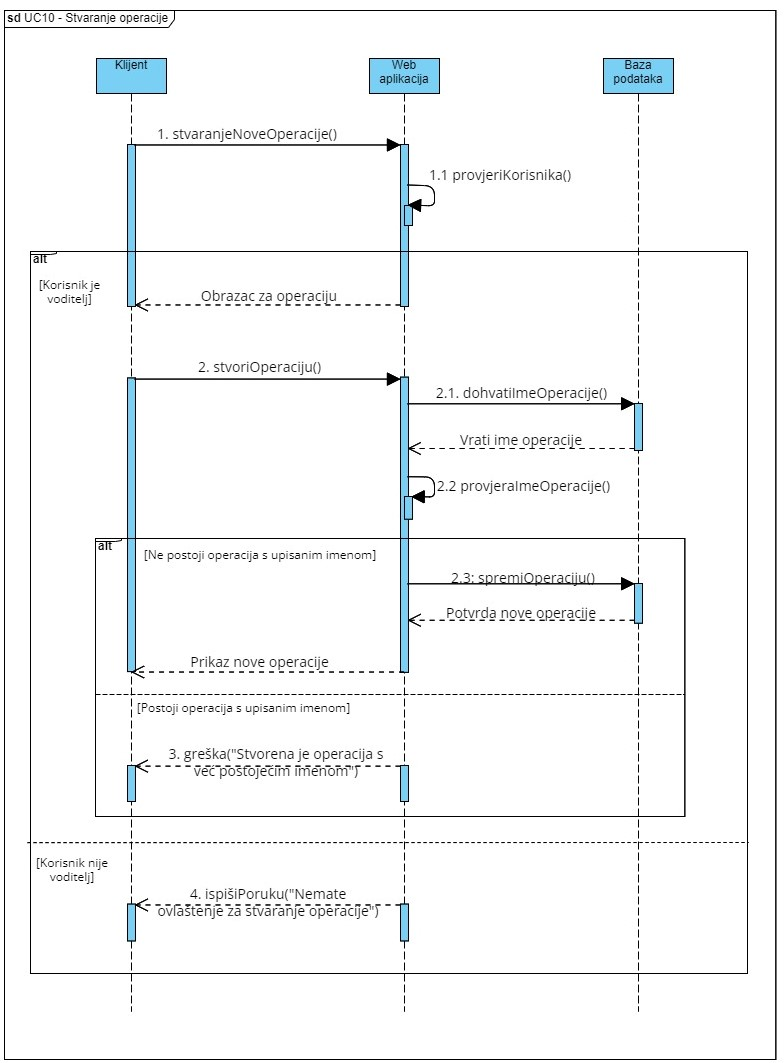
\includegraphics[width=\linewidth]{./dijagrami/StvaranjeOperacije.jpg}
				    \caption{Sekvencijski dijagram za UC10 - Stvaranje operacije}
				    \end{figure}

            	\eject

				\textbf{Obrazac uporabe UC11 - Mijenjanje statusa bloka}

                Klijent šalje zahtjev za prikaz karte. Web poslužitelj prikazuje kartu s opcijama, oviseći o korisniku. Klijent šalje zahtjev za prikaz bloka koji želi uređivati. Sustav dohvaća iz baze taj blok i prikazuje ga klijentu. Klijent šalje zahtjev za promjenu statusa bloka. Web poslužitelj provjerava status bloka te ako je blok aktivan ispisuje poruku da nije dopušteno uređivanje bloka. Ako je blok u statusu "Nezapočeto", klijent šalje zahtjev za promjenu statusa u "Aktivan". Sustav zapisuje status u bazu te prikazuje potvrdu promjene statusa. Ako je blok u statusu "Provjera", kartograf može smatrati da je posao dobro obavljen ili nije. Ukoliko kartograf smatra da posao nije dobro obavljen, šalje zahtjev sustavu za promjenu statusa bloka u "Aktivan" koji se zapisuje u bazu. Ukoliko kartograf smatra da je posao dobro obavljen, potvrđuje blok. Ukoliko su 2 kartografa potvrdila blok, mijenja se status bloka u "Završeno" i zapisuje u bazu. Kad je status bloka aktivan klijent može uređivati blok što se nastavlja u UC12 - Dodavanje građevine u blok. Kad je kartograf gotov s uređivanjem bloka, šalje zahtjev za promjenu statusa u "Provjera". Sustav zapisuje promjenu u bazu te šalje potvrdu.

                \begin{figure}[H] 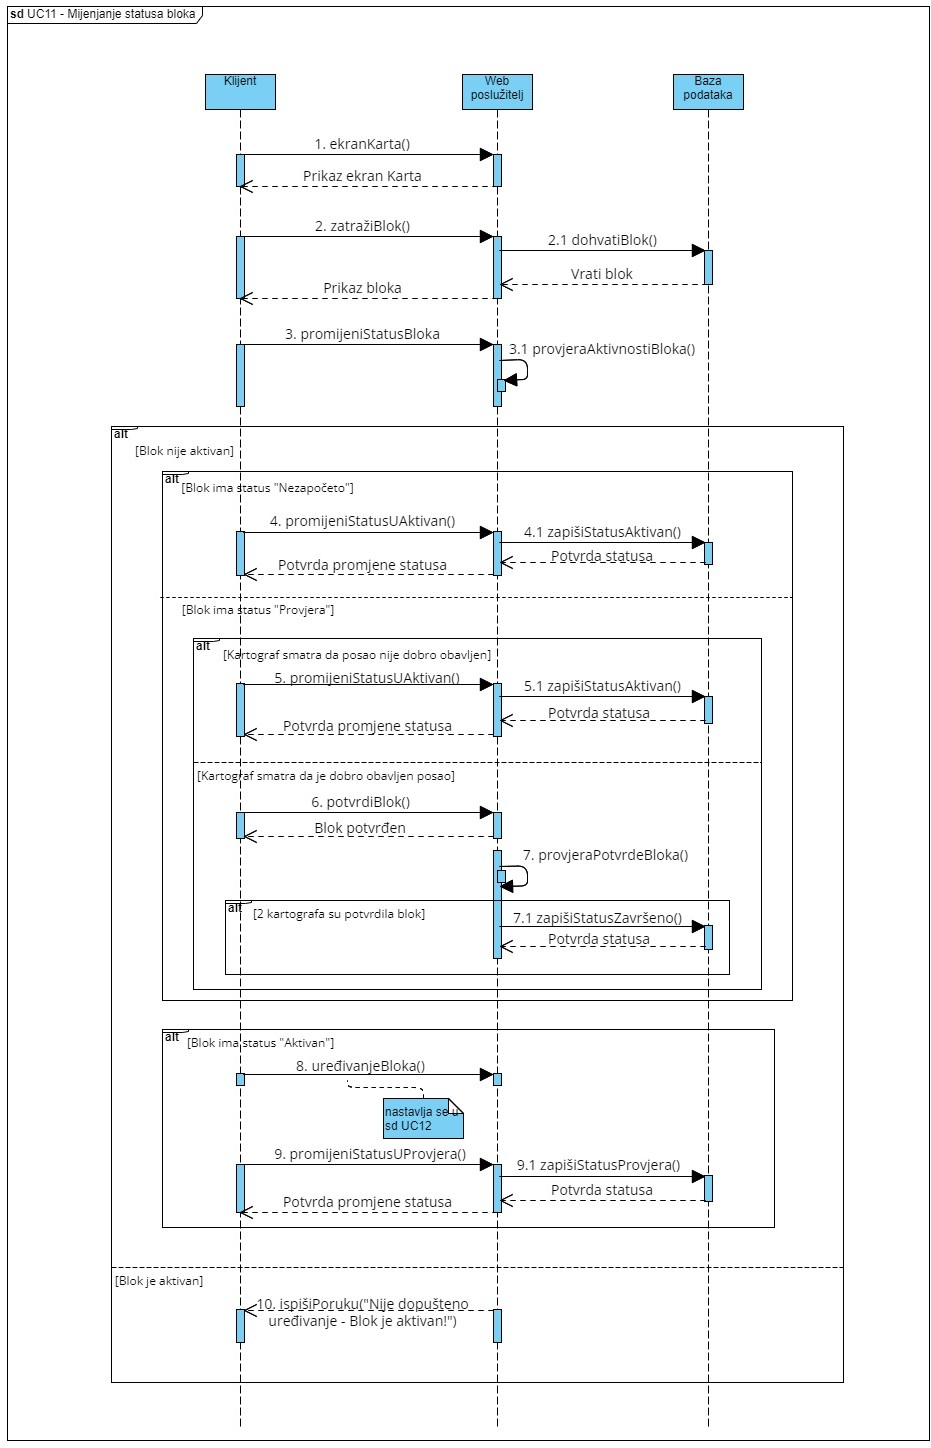
\includegraphics[width=\linewidth]{./dijagrami/MijenjanjeStatusaBloka.jpg}
				    \caption{Sekvencijski dijagram za UC11 - Mijenjanje statusa bloka}
				    \end{figure}
                
                \eject

                \textbf{Obrazac uporabe UC20 - Potvrda registracije}

                Klijent šalje zahtjev za otvaranjem ekrana admin. Sustav provjerava je li korisnik administrator te ako nije, web poslužitelj ispisuje poruku da nema ovlaštenja za pristup Admin pageu. Ukoliko je korisnik administrator, sustav prikazuje ekran Admin. Klijent šalje zahtjev za nepotvrđene registracije. Sustav dohvaća iz baze nepotvrđene korisnike te ih prikazuje. Ako administrator želi potvrditi registraciju, šalje zahtjev sustavu koji zapisuje zapisuje potvrdu korisnika u bazu. Sustav prikazuje potvrdu novog korisnika. Ukoliko administrator ne želi potvrditi registraciju, šalje zahtjev sustavu. Sustav briše korisnika iz baze te šalje potvrdu odbijene registracije. 

                \begin{figure}[H] 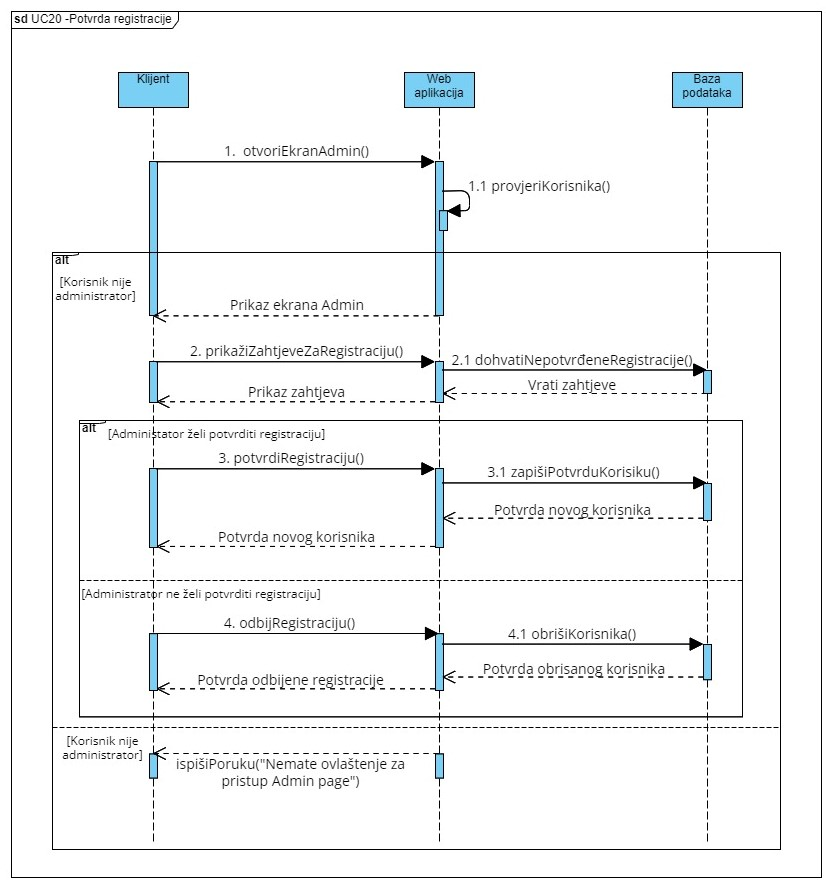
\includegraphics[width=\linewidth]{./dijagrami/PotvrdaRegistracije.jpg}
				    \caption{Sekvencijski dijagram za UC20 - Potvrda registracije}
				    \end{figure}
            \eject
	
		\section{Ostali zahtjevi}
		
			\textbf{\textit{dio 1. revizije}}\\
		 
			 \textit{Nefunkcionalni zahtjevi i zahtjevi domene primjene dopunjuju funkcionalne zahtjeve. Oni opisuju \textbf{kako se sustav treba ponašati} i koja \textbf{ograničenja} treba poštivati (performanse, korisničko iskustvo, pouzdanost, standardi kvalitete, sigurnost...). Primjeri takvih zahtjeva u Vašem projektu mogu biti: podržani jezici korisničkog sučelja, vrijeme odziva, najveći mogući podržani broj korisnika, podržane web/mobilne platforme, razina zaštite (protokoli komunikacije, kriptiranje...)... Svaki takav zahtjev potrebno je navesti u jednoj ili dvije rečenice.}
			 
			 
			 
	